\Aufgabe[ACTL \& LTL\hfill\textbf{(2 Points)}]
\newcommand{\ACTL}{\mathbf{ACTL}}
\newcommand{\LTL}{\mathbf{LTL}}
\newcommand{\CTLstar}{\mathbf{CTL}^*}
\newcommand{\AP}{\mathbf{AP}}
\newcommand{\true}{\mathbf{true}}
\newcommand{\false}{\mathbf{false}}
\newcommand{\trans}{\mathsf{trans}}
Given an LTL formula $\varphi$ in Negation Normal Form, the following function 
$\mathsf{trans} : \LTL \rightarrow \ACTL$ translates $\varphi$ into an ACTL 
formula $\trans(\varphi)$ as follows:
\begin{center}
\begin{tabular}{l|l}
	$\varphi$ & $\trans(\varphi)$\\
	\hline
	$\true$ & $\true$\\
	$\false$ & $\false$\\
	$a$ & $a$\\
	$\neg a$ & $\neg a$\\
	$\varphi_1 \vee \varphi_2$ & $\trans(\varphi_1) \vee \trans(\varphi_2)$\\
	$\varphi_1 \wedge \varphi_2$ & $\trans(\varphi_1) \wedge \trans(\varphi_1)$\\
	$\mathbf{X} \varphi_1$ & $\mathbf{AX}~\trans(\varphi_1)$\\
	$\mathbf{F} \varphi_1$ & $\mathbf{AF}~\trans(\varphi_1)$\\
	$\mathbf{G} \varphi_1$ & $\mathbf{AG}~\trans(\varphi_1)$\\
	$\varphi_1 \mathbf{U} \varphi_2$ & $\mathbf{A}\left[ \trans(\varphi_1)\;\mathbf{U}\;\trans(\varphi_2) \right]$\\
	$\varphi_1 \mathbf{R} \varphi_2$ & $\mathbf{A}\left[ \trans(\varphi_1)\;\mathbf{R}\;\trans(\varphi_2) \right]$\\
\end{tabular}
\end{center}
The semantics of the ``release'' operator $\mathbf{R}$ is defined as follows:
$$M, \pi \models \varphi_1 \mathbf{R} \varphi_2 \stackrel{def}{\Leftrightarrow} \forall j \geq 0. \pi^j \models \varphi_2 \textnormal{ or } \exists i \geq 0. (\pi^i \models \varphi_1) \wedge (\forall k \leq i. \pi^k \models \varphi_2)$$

\paragraph{a)} Show that, for all $\LTL$ formulas $\varphi$ in negation normal form, the $\CTLstar$ 
formula $\trans(\varphi) \Rightarrow \mathbf{A}\varphi$ is a tautology.
\emph{Hint: Show this by showing that $M, s \models \trans(\varphi)$ implies 
$M, s \models \mathbf{A}\varphi$ for all $\LTL$ formulas $\varphi$ in negation normal form, all Kripke 
structures $M$ and all states $s$ in $M$.
Use induction over the structure of~$\varphi$.}\hfill\textbf{(1 Point)}

\textbf{Solution:}

\bigskip

Let $\varphi $ be an arbitrary LTL formula in negation normal form (NNF).
Then the tautologicity of the CTL$^{\ast }$-formula $\mathrm{trans}(\varphi )%
\IMPL\mathbf{A}\varphi $ can be shown by structural induction over all
formulas $\varphi $. Then the satisfaction relation $\models $ for all
Kripke structures $M$ and all states $s\in S$ in $M$ on $M,s\vDash \mathrm{%
trans}(\varphi )\IMPL M,s\vDash \mathbf{A}\varphi $ is defined inductively
as follows:

\newpage

{\small
\textbf{Base case:}

\bigskip

\begin{enumerate}
\item[1.] $\varphi =\mathbf{true}.$

\begin{tabular}{lcl}
$M,s\vDash \mathrm{trans}(\mathbf{true})$ & $\quad \Rightarrow \quad $ & $%
M,s\vDash \mathbf{A\,true}\qquad \text{iff}$ \\ 
iff $M,s\vDash \mathbf{true}$ &  & for every path $\pi \in Paths_{M}(s)$
starting from $s$, \\ 
&  &  $M,\pi \vDash \mathbf{true}\quad $iff \\ 
&  & $s$ is the first state of $\pi $ and $M,s\vDash \mathbf{true}$.%
\end{tabular}

\item[2.] $\varphi =\mathbf{false}.$ Analogously as (1).

\item[3.] $\varphi =a.$

\begin{tabular}{lcl}
$M,s\vDash \mathrm{trans}(a)$ & $\quad \Rightarrow \quad $ & $M,s\vDash 
\mathbf{A}a\qquad \text{iff}$ \\ 
iff $M,s\vDash a$ &  & for every path $\pi \in Paths_{M}(s)$ starting from $s
$,  \\ 
iff $a\in L(s)$. &  & $M,\pi \vDash a\quad $iff \\ 
&  & $s$ is the first state of $\pi $ and $M,s\vDash a\quad $iff\quad $a\in
L(s)$.%
\end{tabular}
\end{enumerate}

\bigskip

\textbf{Induction step:}

\bigskip

\begin{enumerate}
\item[4.] $\varphi =\lnot a.$

\begin{tabular}{lcl}
$M,s\vDash \mathrm{trans}(\lnot a)$ & $\quad \Rightarrow \quad $ & $%
M,s\vDash \mathbf{A\lnot }a\qquad \text{iff}$ \\ 
iff $M,s\vDash \lnot a$ &  & for every path $\pi \in Paths_{M}(s)$ starting
from $s$, \\ 
iff $M,s\nvDash a$. &  &  $M,\pi \vDash \lnot a\quad $iff \\ 
&  & $s$ is the first state of $\pi $ and $M,s\nvDash a$.%
\end{tabular}

\item[5.] $\varphi =(\varphi _{1}\OR\varphi _{2}).$

\begin{tabular}{lcl}
$M,s\vDash \mathrm{trans}(\varphi _{1}\OR\varphi _{2})$ & $\quad \Rightarrow
\quad $ & $M,s\vDash \mathbf{A}(\varphi _{1}\OR\varphi _{2})\qquad \text{iff}
$ \\ 
iff$\quad M,s\vDash \mathrm{trans}(\varphi _{1})\OR M,s\vDash \mathrm{trans}%
(\varphi _{2})$ &  & $M,s\vDash \mathbf{A}\varphi _{1}\OR M,s\vDash \mathbf{A%
}\varphi _{2}\qquad \text{iff}$ \\ 
iff$\quad M,s\vDash \mathrm{trans}(\varphi _{1})$\quad or$\quad M,s\vDash 
\mathrm{trans}(\varphi _{2})$ &  & $M,s\vDash \mathbf{A}\varphi _{1}$\quad or%
$\quad M,s\vDash \mathbf{A}\varphi _{2}\qquad \text{iff}$ \\ 
iff$\quad M,s\vDash \mathbf{A}\varphi _{1}$\quad or$\quad M,s\vDash \mathbf{A%
}\varphi _{2}$ &  & $\Forall\pi \in Paths_{M}(s)$ starting from $s$, \\ 
iff$\quad \Forall\pi \in Paths_{M}(s)$ starting from $s$, &  & s.t. $M,\pi
\vDash \varphi _{1}\quad $or$\quad M,\pi \vDash \varphi _{2}\qquad $iff \\ 
s.t. $M,\pi \vDash \varphi _{1}\quad $or$\quad M,\pi \vDash \varphi _{2}$ & 
& $\Forall\pi \in Paths_{M}(s)$, $s$ is the first \\ 
iff$\quad \Forall\pi \in Paths_{M}(s)$, $s$ is the first &  & state of $\pi $%
, s.t. $M,s\vDash \varphi _{1}$ or $M,s\vDash \varphi _{2}$. \\ 
state of $\pi $, s.t. $M,s\vDash \varphi _{1}$ or $M,s\vDash \varphi _{2}$.
&  & 
\end{tabular}

\item[6.] $\varphi =(\varphi _{1}\AND\varphi _{2}).$ Analogously as (5).

\item[7.] $\varphi =\mathbf{X}\varphi _{1}.$

\begin{tabular}{lcl}
$M,s\vDash \mathbf{AX}\,\mathrm{trans}(\varphi _{1})$ & $\quad \Rightarrow
\quad $ & $M,s\vDash \mathbf{A(X}\varphi _{1})\qquad \text{iff}$ \\ 
iff$\quad \Forall\pi \in Paths_{M}(s)$ starting from $s$, &  & for every
path $\pi \in Paths_{M}(s)$ starting \\ 
$M,\pi \vDash \mathbf{X}\,\mathrm{trans}(\varphi _{1})$ &  &  from $s$, $%
M,\pi \vDash \mathbf{X}\varphi _{1}\qquad $iff \\ 
iff$\quad M,\pi ^{1}\vDash \mathrm{trans}(\varphi _{1})$ &  & $M,\pi
^{1}\vDash \varphi _{1}\qquad $iff \\ 
iff$\quad \pi $ starts at $s_{1}$, s.t. $M,s_{1}\vDash \mathrm{trans}%
(\varphi _{1})$ &  & $\Forall\pi \in Paths_{M}(s_{1})$, $\pi $ starts at $%
s_{1}$, \\ 
iff$\quad M,s_{1}\vDash \mathbf{A}\varphi _{1}$ &  & s.t. $M,s_{1}\vDash
\varphi _{1}$. \\ 
iff$\quad \Forall\pi \in Paths_{M}(s_{1})$ starting &  &  \\ 
from $s_{1}$, $M,\pi \vDash \varphi _{1}$ &  &  \\ 
iff$\quad s_{1}$ is the first state of $\pi $, s.t. $M,s_{1}\vDash \varphi
_{1}$. &  & 
\end{tabular}

\item[8.] $\varphi =\mathbf{F}\varphi _{1}.$

\begin{tabular}{lcl}
$M,s\vDash \mathbf{AF}\,\mathrm{trans}(\varphi _{1})$ & $ \Rightarrow
\quad $ & $M,s\vDash \mathbf{A(F}\varphi _{1})\qquad \text{iff}$ \\ 
iff$\quad \Forall\pi \in Paths_{M}(s)$ starting from $s$, &  & for every
path $\pi \in Paths_{M}(s)$ starting \\ 
$M,\pi \vDash \mathbf{F}\,\mathrm{trans}(\varphi _{1})$ &  &  from $s$, $%
M,\pi \vDash \mathbf{F}\varphi _{1}\qquad $iff \\ 
iff$\quad \Exists k\geq 0$ s.t. $M,\pi ^{k}\vDash \mathrm{trans}(\varphi
_{1})$ &  & $\Exists k\geq 0$ s.t. $M,\pi ^{k}\vDash \varphi _{1}\qquad $iff
\\ 
iff$\quad \pi $ starts at $s_{k}$, s.t. $M,s_{k}\vDash \mathrm{trans}%
(\varphi _{1})$ &  & $s_{k}$ is the first state of $\pi $, s.t. $%
M,s_{k}\vDash \varphi _{1}$. \\ 
iff$\quad M,s_{k}\vDash \mathbf{A}\varphi _{1}$ &  &  \\ 
iff$\quad \Forall\pi \in Paths_{M}(s_{k})$ starting from $s_{k}$, &  &  \\ 
$M,\pi \vDash \varphi _{1}$ &  &  \\ 
iff$\quad s_{k}$ is the first state of $\pi $, s.t. $M,s_{k}\vDash \varphi
_{1}$. &  & 
\end{tabular}

\item[9.] $\varphi =\mathbf{G}\varphi _{1}.$

\begin{tabular}{lcl}
$M,s\vDash \mathbf{AG}\,\mathrm{trans}(\varphi _{1})$ & $ \Rightarrow
\quad $ & $M,s\vDash \mathbf{A(G}\varphi _{1})\qquad \text{iff}$ \\ 
iff$\quad \Forall\pi \in Paths_{M}(s)$ starting from $s$, &  & for every
path $\pi \in Paths_{M}(s)$ starting \\ 
$M,\pi \vDash \mathbf{G}\,\mathrm{trans}(\varphi _{1})$ &  &  from $s$, $%
M,\pi \vDash \mathbf{G}\varphi _{1}\qquad $iff \\ 
iff$\quad \Forall i\geq 0$, $M,\pi ^{i}\vDash \mathrm{trans}(\varphi _{1})$
&  & $\Forall i\geq 0$, $M,\pi ^{i}\vDash \varphi _{1}\qquad $iff \\ 
iff$\quad \Forall i\geq 0$, $\pi $ at $s_{i}$, $M,s_{i}\vDash \mathrm{trans}%
(\varphi _{1})$ &  & $\Forall i\geq 0$, $s_{i}$ is a state in $\pi $ and $%
M,s_{i}\vDash \varphi _{1}$. \\ 
iff$\quad \Forall i\geq 0$, $M,s_{i}\vDash \mathbf{A}\varphi _{1}$ &  &  \\ 
iff$\quad \Forall i\geq 0$ and $\Forall\pi \in Paths_{M}(s_{i})$ &  &  \\ 
starting from $s_{i}$,$M,\pi \vDash \varphi _{1}$ &  &  \\ 
iff$\quad \Forall i\geq 0$, $s_{i}$ is a state in $\pi $ and $M,s_{i}\vDash
\varphi _{1}$. &  & 
\end{tabular}

\item[10.] $\varphi =(\varphi _{1}\mathbf{U}\varphi _{2}).$

{\scriptsize
\begin{tabular}{lcl}
$M,s\vDash \mathbf{A[}\mathrm{trans}(\varphi _{1})\,\mathbf{U\,}\mathrm{trans%
}(\varphi _{2})]$ & $ \Rightarrow $ & $M,s\vDash \mathbf{A}%
(\varphi _{1}\mathbf{U}\varphi _{2})\qquad \text{iff}$ \\ 
iff$\quad \Forall\pi \in Paths_{M}(s)$ starting from $s$, $\Exists k\geq 0$
s.t. &  & for every path $\pi \in Paths_{M}(s)$ starting from $s$, \\ 
&  & $M,\pi \vDash (\varphi _{1}\mathbf{U}\varphi _{2})\qquad $iff \\ 
$M,\pi ^{k}\vDash \mathrm{trans}(\varphi _{2})$ and $\Forall j,0\leq j<k$, $%
M,\pi ^{j}\vDash \mathrm{trans}(\varphi _{1})$ &  & $\Exists k\geq 0$ s.t. $%
\Forall\pi \in Paths_{M}(s_{k})$ \\ 
iff$\quad \Exists k\geq 0$ s.t. $\pi $ at $s_{k}$, $M,s_{k}\vDash \mathrm{%
trans}(\varphi _{2})$ and &  & starting from $s_{k}$, $M,\pi \vDash \varphi
_{2}$ and $\Forall j,0\leq j<k$ \\ 
$\Forall j,0\leq j<k$, $\pi $ starts at $s_{j}$ s.t. $M,s_{j}\vDash \mathrm{%
trans}(\varphi _{1})$ &  & s.t. $\Forall\pi \in Paths_{M}(s_{j})$ starting
from $s_{j}$, \\ 
iff$\quad \Exists k\geq 0$ s.t. $M,s_{k}\vDash \mathbf{A}\varphi _{2}$ and $%
\Forall j,0\leq j<k$, &  & $M,\pi \vDash \varphi _{1}\qquad $iff \\ 
$M,s_{j}\vDash \mathbf{A}\varphi _{1}$ &  & $\Exists k\geq 0$ s.t. $s_{k}$
is the first state in $\pi $, $M,s_{k}\vDash \varphi _{2}$ and \\ 
iff$\quad \Exists k\geq 0$ s.t. $\Forall\pi \in Paths_{M}(s_{k})$ starting
from $s_{k}$, &  & $\Forall j,0\leq j<k$, $s_{j}$ is a state in $\pi $ s.t. $%
M,s_{j}\vDash \varphi _{2}$. \\ 
$M,\pi \vDash \varphi _{2}$ and $\Forall j,0\leq j<k$ s.t. $\Forall\pi \in
Paths_{M}(s_{j})$ &  &  \\ 
starting from $s_{j}$, $M,\pi \vDash \varphi _{1}$ &  &  \\ 
iff$\quad \Exists k\geq 0$ s.t. $s_{k}$ is the first state in $\pi $, $%
M,s_{k}\vDash \varphi _{2}$ and &  &  \\ 
$\Forall j,0\leq j<k$, $s_{j}$ is a state in $\pi $ s.t. $M,s_{j}\vDash
\varphi _{2}$. &  & 
\end{tabular}
}

\item[11.] $\varphi =(\varphi _{1}\mathbf{R}\varphi _{2}).$

{\scriptsize
\begin{tabular}{lcl}
$M,s\vDash \mathbf{A[}\mathrm{trans}(\varphi _{1})\,\mathbf{R\,}\mathrm{trans%
}(\varphi _{2})]$ & $ \Rightarrow  $ & $M,s\vDash \mathbf{A}%
(\varphi _{1}\mathbf{R}\varphi _{2})\qquad \text{iff}$ \\ 
iff$\quad \Forall\pi \in Paths_{M}(s)$ starting from $s$ and $\Forall j\geq 0
$, &  & for every path $\pi \in Paths_{M}(s)$ starting \\ 
&  &  from $s$, $M,\pi \vDash (\varphi _{1}\mathbf{R}\varphi _{2})\qquad $iff
\\ 
$M,\pi ^{j}\vDash \mathrm{trans}(\varphi _{2})$ or $(\Exists i\geq 0$ s.t. $%
M,\pi ^{i}\vDash \mathrm{trans}(\varphi _{1})$ and &  & $\Forall j\geq 0$
s.t. $\Forall\pi \in Paths_{M}(s_{j})$ starting \\ 
$\Forall k\leq i$, $M,\pi ^{k}\vDash \mathrm{trans}(\varphi _{2}))$ &  & 
from $s_{j}$, $M,\pi \vDash \varphi _{2}$ or $(\Exists i\geq 0$ s.t. \\ 
iff$\quad \Forall j\geq 0$ s.t. $\pi $ starts at $s_{j}$ s.t. $M,s_{j}\vDash 
\mathrm{trans}(\varphi _{2})$ or &  & $\Forall\pi \in Paths_{M}(s_{i})$, $%
M,\pi \vDash \varphi _{1}$ and \\ 
$(\Exists i\geq 0$ s.t. $\pi $ at $s_{i}$, $M,s_{i}\vDash \mathrm{trans}%
(\varphi _{1})$ and $\Forall k\leq i$, &  & $\Forall k\leq i$ and $\Forall%
\pi \in Paths_{M}(s_{k})$, \\ 
$\pi $ at $s_{k}$ s.t. $M,s_{k}\vDash \mathrm{trans}(\varphi _{2}))$ &  &  $%
M,\pi \vDash \varphi _{2})$\qquad iff \\ 
iff$\quad \Forall j\geq 0$ s.t. $M,s_{j}\vDash \mathbf{A}\varphi _{2}$ or $(%
\Exists i\geq 0$ s.t. &  & $\Forall j\geq 0$, $s_{j}$ is a state in $\pi $
s.t. $M,s_{j}\vDash \varphi _{2}$ or \\ 
$M,s_{i}\vDash \mathbf{A}\varphi _{1}$and $\Forall k\leq i$, $M,s_{k}\vDash 
\mathbf{A}\varphi _{2})$ &  & $(\Exists i\geq 0$ and $s_{i}$ is the first
state in $\pi $ s.t. \\ 
iff$\quad \Forall j\geq 0$ s.t. $\Forall\pi \in Paths_{M}(s_{j})$ starting
from $s_{j}$, &  & $M,s_{i}\vDash \varphi _{1}$ and $\Forall k\leq i$, $s_{k}
$ is a state in $\pi $ s.t. \\ 
$M,\pi \vDash \varphi _{2}$ or $(\Exists i\geq 0$ s.t. $\Forall\pi \in
Paths_{M}(s_{i})$, &  & $M,s_{k}\vDash \varphi _{2})$. \\ 
$M,\pi \vDash \varphi _{1}$ and $\Forall k\leq i$ and $\Forall\pi \in
Paths_{M}(s_{k})$, $M,\pi \vDash \varphi _{2})$ &  &  \\ 
iff$\quad \Forall j\geq 0$, $s_{j}$ is a state in $\pi $ s.t. $M,s_{j}\vDash
\varphi _{2}$ or $(\Exists i\geq 0$ &  &  \\ 
and $s_{i}$ is the first state in $\pi $ s.t. $M,s_{i}\vDash \varphi _{1}$
and $\Forall k\leq i$, &  &  \\ 
$s_{k}$ is a state in $\pi $ s.t. $M,s_{k}\vDash \varphi _{2})$. &  & 
\end{tabular}
}
\end{enumerate}
}

\paragraph{b)} Show that, in general, $M, s \models \varphi$ does not imply $M, s \models \trans(\varphi)$.
\emph{Hint: Give a Kripke structure $M$ and an $\LTL$ formula $\varphi$ such that $M, s \models \varphi$ and $M, s \not\models \trans(\varphi)$. Discuss why $M, s \models \varphi$ and $M, s \not\models \trans(\varphi)$ holds on $M$ and the given state $s$ in $M$.}\\{\color{white} whitespace}\hfill\textbf{(1 Point)}

\textbf{Solution:}
\bigskip

In general, the other direction of the implication such that $M,s\vDash
\varphi \IMPL M,s\vDash \mathrm{trans}(\varphi )$, does not always hold,
i.e. the implication is not valid for all Kripke models and all states $s$
in $M$. It can be shown, that both logics, ACTL and LTL\ have different
power of expressiveness. I.e.

\begin{definition}
Let $\mathbf{\phi }$ be a ACTL\ formula, and $\varphi $ the LTL formula that
is obtained by eleminating all path quantifiers in $\mathbf{\phi }$. Then,%
\begin{equation*}
\mathbf{\phi }\equiv \varphi \text{ or there does not exist any LTL\ formula
that is equivalent to }\mathbf{\phi }\text{.}
\end{equation*}
\end{definition}

Then following ACTL\ formula $\mathbf{AFAG}a$ and the corresponding LTL\
formula $\mathbf{FG}a$, obtained by the above definition, are not equivalent.
\bigskip\\

\textit{Proof:} Consider following Kripke structure $M$ over $AP=\{a\}$:

\begin{center}
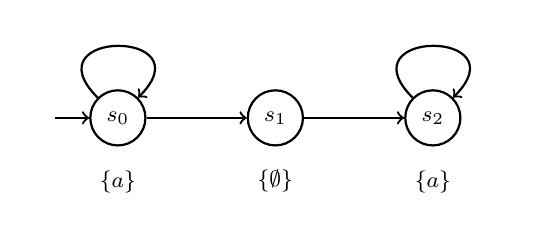
\begin{tikzpicture}[->,scale=1,label distance=0mm]
	\tikzstyle{every node}=[draw,shape=circle,minimum size=7mm,font=\footnotesize];
    \tikzstyle{every path}=[draw,thick];
    
    \node at (0, 0)  (s0) [label=below:${ \{a\} }$] {$s_0$};
    \node at (2, 0) (s1) [label=below:${ \{\emptyset\} }$] {$s_1$};
    \node at (4, 0)  (s2) [label=below:${ \{a\} }$] {$s_2$};

    \draw (-0.8, 0) to (s0);
    \draw (s0) to (s1);
    \draw (s1) to (s2);
	\draw (s0) .. controls +(135:16mm) and +(45:16mm) .. (s0);
	\draw (s2) .. controls +(135:16mm) and +(45:16mm) .. (s2);
\end{tikzpicture}
\end{center}

The LTL\ formula $\mathbf{FG}a$ expresses the property that there is some
state from which $a$ will hold forever. The initial state $s_{0}$ in $M$
satisfies $\mathbf{FG}a$, since each path starting in $s_{0}$ will
eventually remain forever in one of the two states $s_{0}$ or $s_{2}$.
Whereas the ACTL formula $\mathbf{AFAG}a$ does not hold in $s_{0}$, since
the semantics of $\mathbf{AFAG}a$ is different, i.e. it expresses that on
every computation path there is eventually some state $s_{j},j\geq 0$, such
that $M,s_{j}\vDash \mathbf{AG}a$ and for $\mathbf{AG}a$ it entails that for
any path $\pi $, there exists some state $s_{j}$, such that all reachable
states from $s_{j}$ satisfy $a$.

Let $s_{0}^{w}$ be a path starting in $s_{0}$. Then it follows that $%
M,s_{0}^{w}\nvDash \mathbf{FAG}a$, since $M,s_{0}\nvDash \mathbf{AG}a$%
, because the path $\pi =s_{0}^{\ast }s_{1}s_{2}^{w}$ passes \ through a $%
\lnot a$-state in $s_{1}$. Thus, $s_{0}^{w}$ will never reach a state
satisfying $\mathbf{AG}a$, i.e. $M,s_{0}^{w}\nvDash \mathbf{FAG}a$, and
hence $M,s_{0}\nvDash \mathbf{AFAG}a$.

